\paragraph*{}
  Des plasmas qui composent les nébuleuses aux arrivées d'eau de nos maisons en passant par les systèmes de
  refroidissement des centrales nucléaires et le flux sanguin alimentant notre métabolisme.
  Les fluides composent la majorité de la matière visible dans notre univers \cite{plasma}.
  La dynamique de ces fluides sont décrits par une équation rédigée au milieu XIXe siècle \cite{wiki:NS}.
  Fruit de la collaboration de générations de physiciens, les équations de \NS{} sont toujours aujourd'hui au cœur de
  nombreuses problématiques.
  La question de l'existence et de la régularité des solutions des équations de \NS{} en 3D constitue encore aujourd'hui 
  un problème ouvert et est l'un des problèmes du prix du millénaire de l'institut de mathématique de Clay 
  \cite{wiki:Mil}.

\paragraph*{}
  À défaut d'une solution analytique, c'est dès la première moitié du XXe siècle que les physiciens développent les
  premières méthodes de résolutions numériques des équations de \NS{} \cite{Hunt1998}.
  Depuis l'apparition des premiers ordinateurs, on a assisté à l'émergence de nombreuses méthodes numériques de résolution 
  de dynamique des fluides.
  La branche de la physique utilisant et étudiant ces méthodes et nommée \emph{Computational fluid dynamic} aussi abrégée 
  en CFD.
  La méthode qui nous intéresse ce nome la méthode de Boltzmann sur réseau plus couramment abrégée par LBM pour 
  \emph{Lattice Boltzmann Methods}.

\paragraph*{}
  Les LBM apparaissent au milieu des années 1980 \cite{D'HUMIERES1985, d_Humi_res_1986, PhysRevLett.56.1505, 
  DHUMIERES2009821} depuis lors cette méthode gagne en popularité comme l'illustre les 
  figures\footnote{La méthodologie permettent d'obtenir ces valeurs est critiquable néanmoins elles montrent une tendance 
  générale.} \ref{fig:LBM}, \ref{fig:CFD} et \ref{fig:ratio}.

\begin{figure}[htp]
  \center
  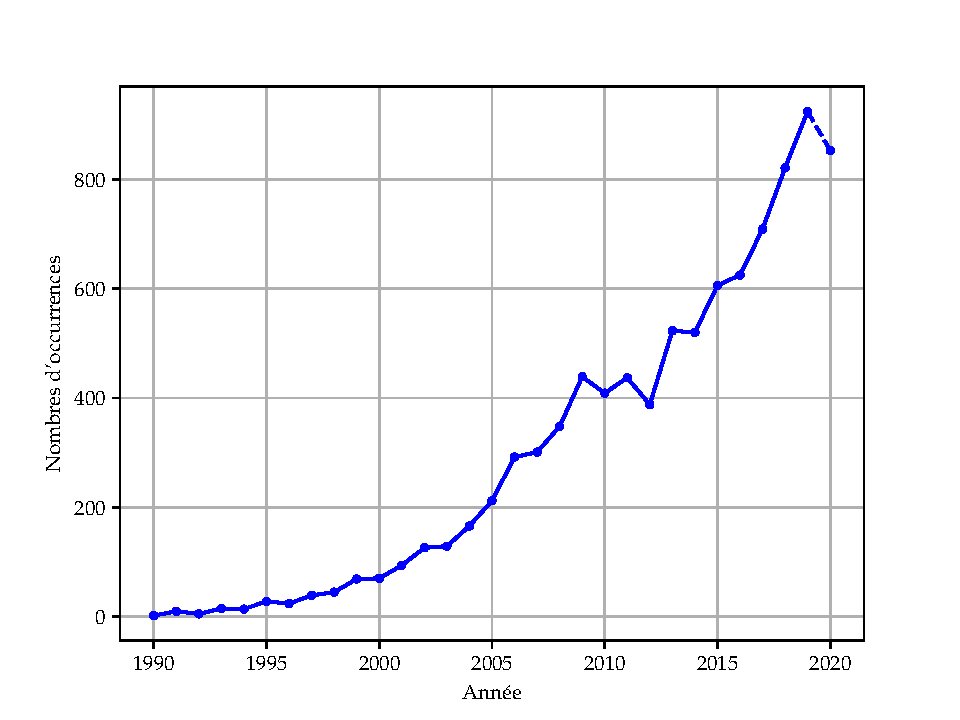
\includegraphics[width=\linewidth]{LBM} 
  \caption{Évolution du nombre de publication référencée dans \href{https://scholar.google.fr/}{Google Scholar} 
              possédant l'occurence <<Lattice Boltzmann Methods>> au cours de ces 30 dernières années.}
  \label{fig:LBM}
\end{figure}

\begin{figure}[htp]
  \center
  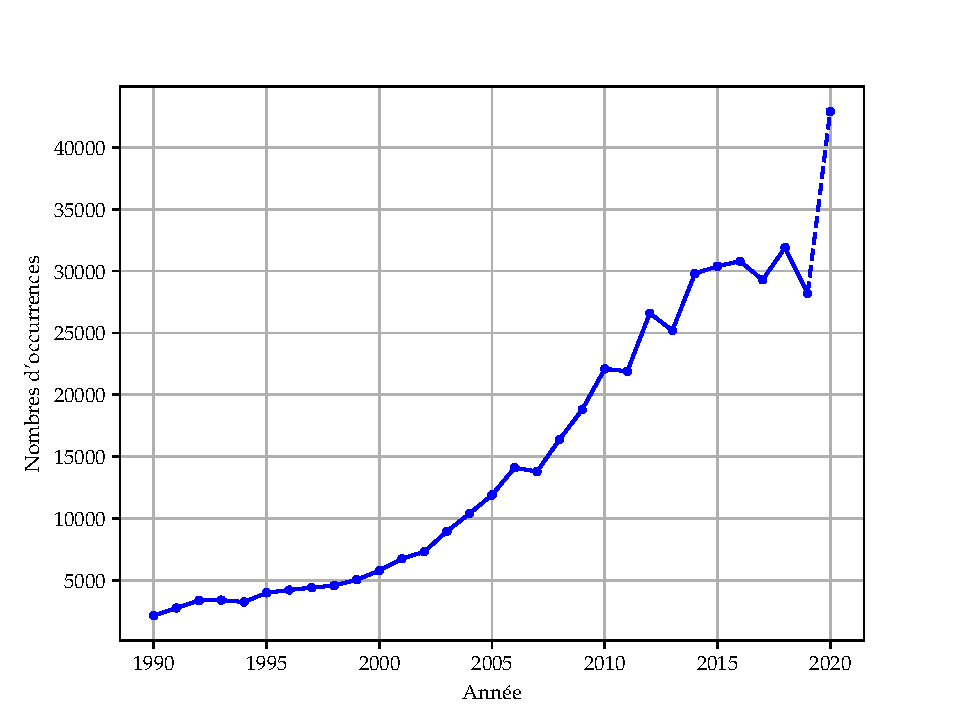
\includegraphics[width=\linewidth]{CFD} 
  \caption{Évolution du nombre de publication référencée dans \href{https://scholar.google.fr/}{Google Scholar} 
              possédant l'occurence <<Computational fluid dynamics>> au cours de ces 30 dernières années.}
  \label{fig:CFD}
\end{figure}

\begin{figure}[htp]
  \center
  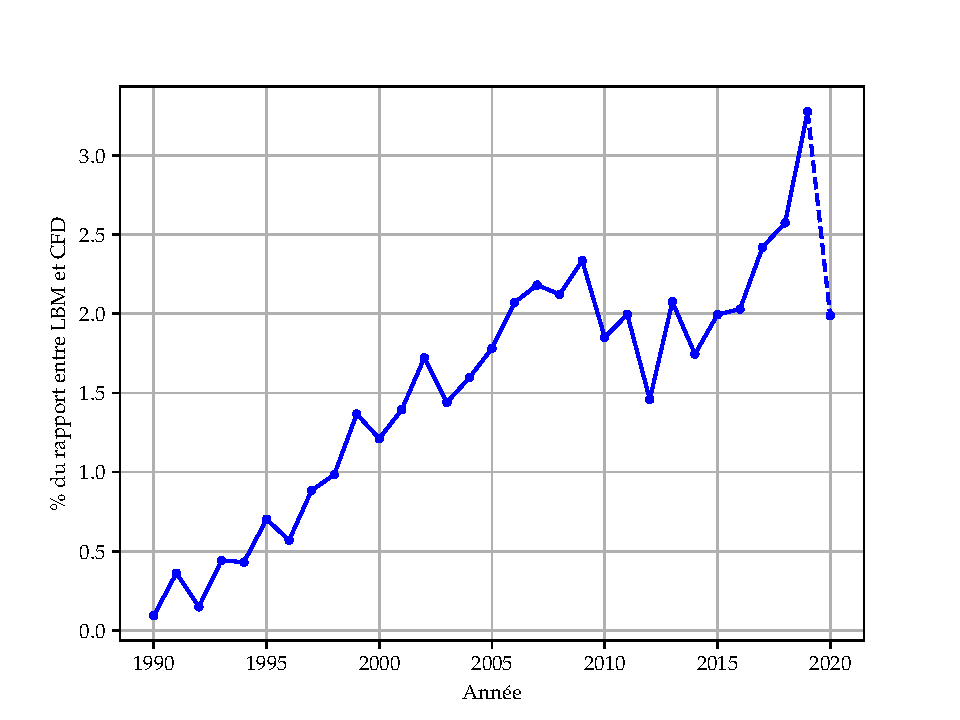
\includegraphics[width=\linewidth]{LBMoCFD} 
  \caption{Rapport en pourcentage entre la figure \ref{fig:LBM} et la figure \ref{fig:CFD}.}
  \label{fig:ratio}
\end{figure}
  
  Ce succès peut s'expliquer par le fait que les LBM profitent de différentes propriétés intéressantes :
  \begin{itemize}
    \itemb Polyvalence :\\
    \emph{Les LBM peuvent être utilisées sur des problèmes très différents (aérodynamiques, médicaux, \dots{}).}

    \itemb Complexité :\\
    \emph{Les LBM peuvent facilement simuler des objets a géométries complexes et peuvent inclure des interactions entre
    plusieurs fluides ainsi que de la thermodynamique et d'autres forces en tout genres.}

    \itemb Parallélisation:\\
    \emph{Les LBM profitent de pleinement des accélérations permises par les architectures 
    \href{https://fr.wikipedia.org/wiki/Microprocesseur_multi-c\%C5\%93ur}{multicores} et 
    \href{https://fr.wikipedia.org/wiki/Processeur_graphique}{GPU} les simulations peuvent donc être déployées sur 
    différents \href{https://fr.wikipedia.org/wiki/Superordinateur}{HPC} et
    \href{https://fr.wikipedia.org/wiki/Grappe_de_serveurs}{clusters de calculs}.}
    
    \itemb Pas d'inconnues:\\
    \emph{Les LBM contrairement a d'autres méthodes plus communes résolvant directement \NS{} possède toutes les quantités
    nécessaires à la résolution déjà définies\footnote{Elle ne demande donc pas (par exemple) de résoudre les équations de
    poissons pour la pression à chaque itération.} et ce de manière locale\footnote{Ce qui explique le fait que les LBM 
    sont hautement parallélisable.}.}
  \end{itemize}
  
   Il est à noter que ces qualités sont inhérentes aux LBM et ne demandes pas de modifications majeures pour êtres 
   implémentées\footnote{À comprendre que l'algorithme de résolution reste le même.}.
   